\section{Validation des résultats}

\`A ce stade d'avancement du projet, la validation des résultats n'est pas totale. Cependant quelques mesures ont été effectuées et un script permet de comparer le comportement de la bibliothèque implémentée par rapport à \texttt{p\_thread}.

\subsection{Passage des tests fournis}

\paragraph{}
Tous les tests fournis par M. Goglin fonctionnent avec la bibliothèque implémentée \texttt{thread.so}. Aucune erreur mémoire ne se présente pour ces tests (aucune fuite mémoire, aucune erreur de lecture). \textsf{Valgrind} détecte cependant un changement de pile (et émet un avertissement). Mais cette manipulation est maîtrisée : elle permet en effet de désallouer correctement la pile dans le test \texttt{12-join-main}.

\paragraph{}
Les résultats sont ensuite comparés à ceux de \texttt{p\_thread} afin de les valider. Le script \texttt{run\_tests.sh} permet de lancer tous les tests avec chacune des deux bibliothèques et affiche un \texttt{diff} pour l'affichage des tests, ainsi qu'un autre pour les résultats de \textsf{Valgrind}.

\subsection{Comparaison avec \texttt{p\_thread}}

\paragraph{}
Une comparaison de performance avec \texttt{p\_thread} peut sembler controversable puisque nous n'utilisons qu'une seul thread noyau. Les temps de création et destruction des threads seront donc inférieurs pour \texttt{thread.so}, en revanche les threads ne s'exécuteront pas en parallèle donc les temps de calculs peuvent être plus longs.

\paragraph{}
Ainsi la comparaison des temps sur les tests 31, 32 et 51 (respectivement création de threads et yield, création récursive de threads et yield et enfin fibonacci) devraient donc donner les résultats suivants : 31 et 32 plus rapides pour \texttt{thread.so}, 51 plus rapide pour \texttt{p\_thread}.
\\
\begin{figure}[!h]
  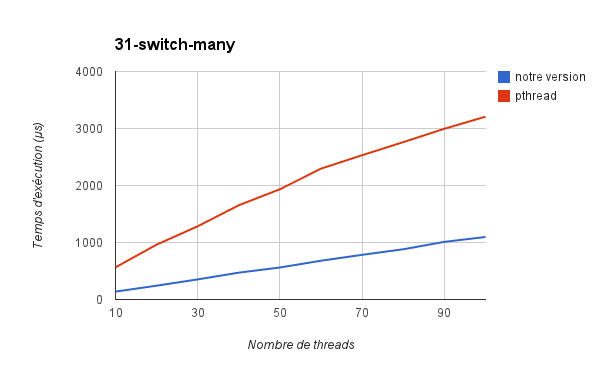
\includegraphics[scale=0.5]{31.png}
\end{figure}

\begin{figure}[!h]
  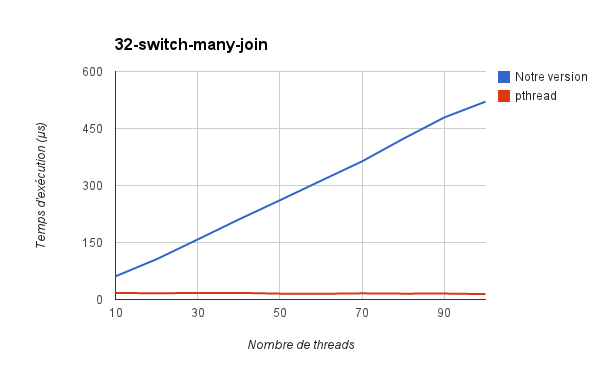
\includegraphics[scale=0.5]{32.png}
\end{figure}

\begin{figure}[!h]
  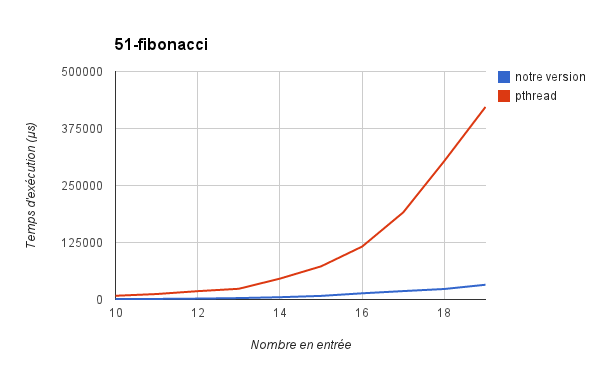
\includegraphics[scale=0.5]{51.png}
\end{figure}

Tous les tests ne sont toutefois pas en accord avec les prévisions faites : notamment en ce qui concerne les tests 32 et 51.
